\subsubsection{\gls{KA}}

\textbf{Ansvar} \\
\gls{KA} er den del af systemet hvor produktkataloget bliver vist og benyttet til salg af produkter. Her i bliver vist en liste/indkøbskurv med de produkter som en evt. kunde ønsker at købe, samt dannet salgskvitteringer for gennemførte salg. Produktkataloget bliver hentet ved en forespørgsel til \gls{CS} og \gls{KA} ved derved intet om oprettelse og redigering af de produkter som den fremviser. \\

\textbf{Sekvensdiagram}
\begin{figure}[H]
	\centering
	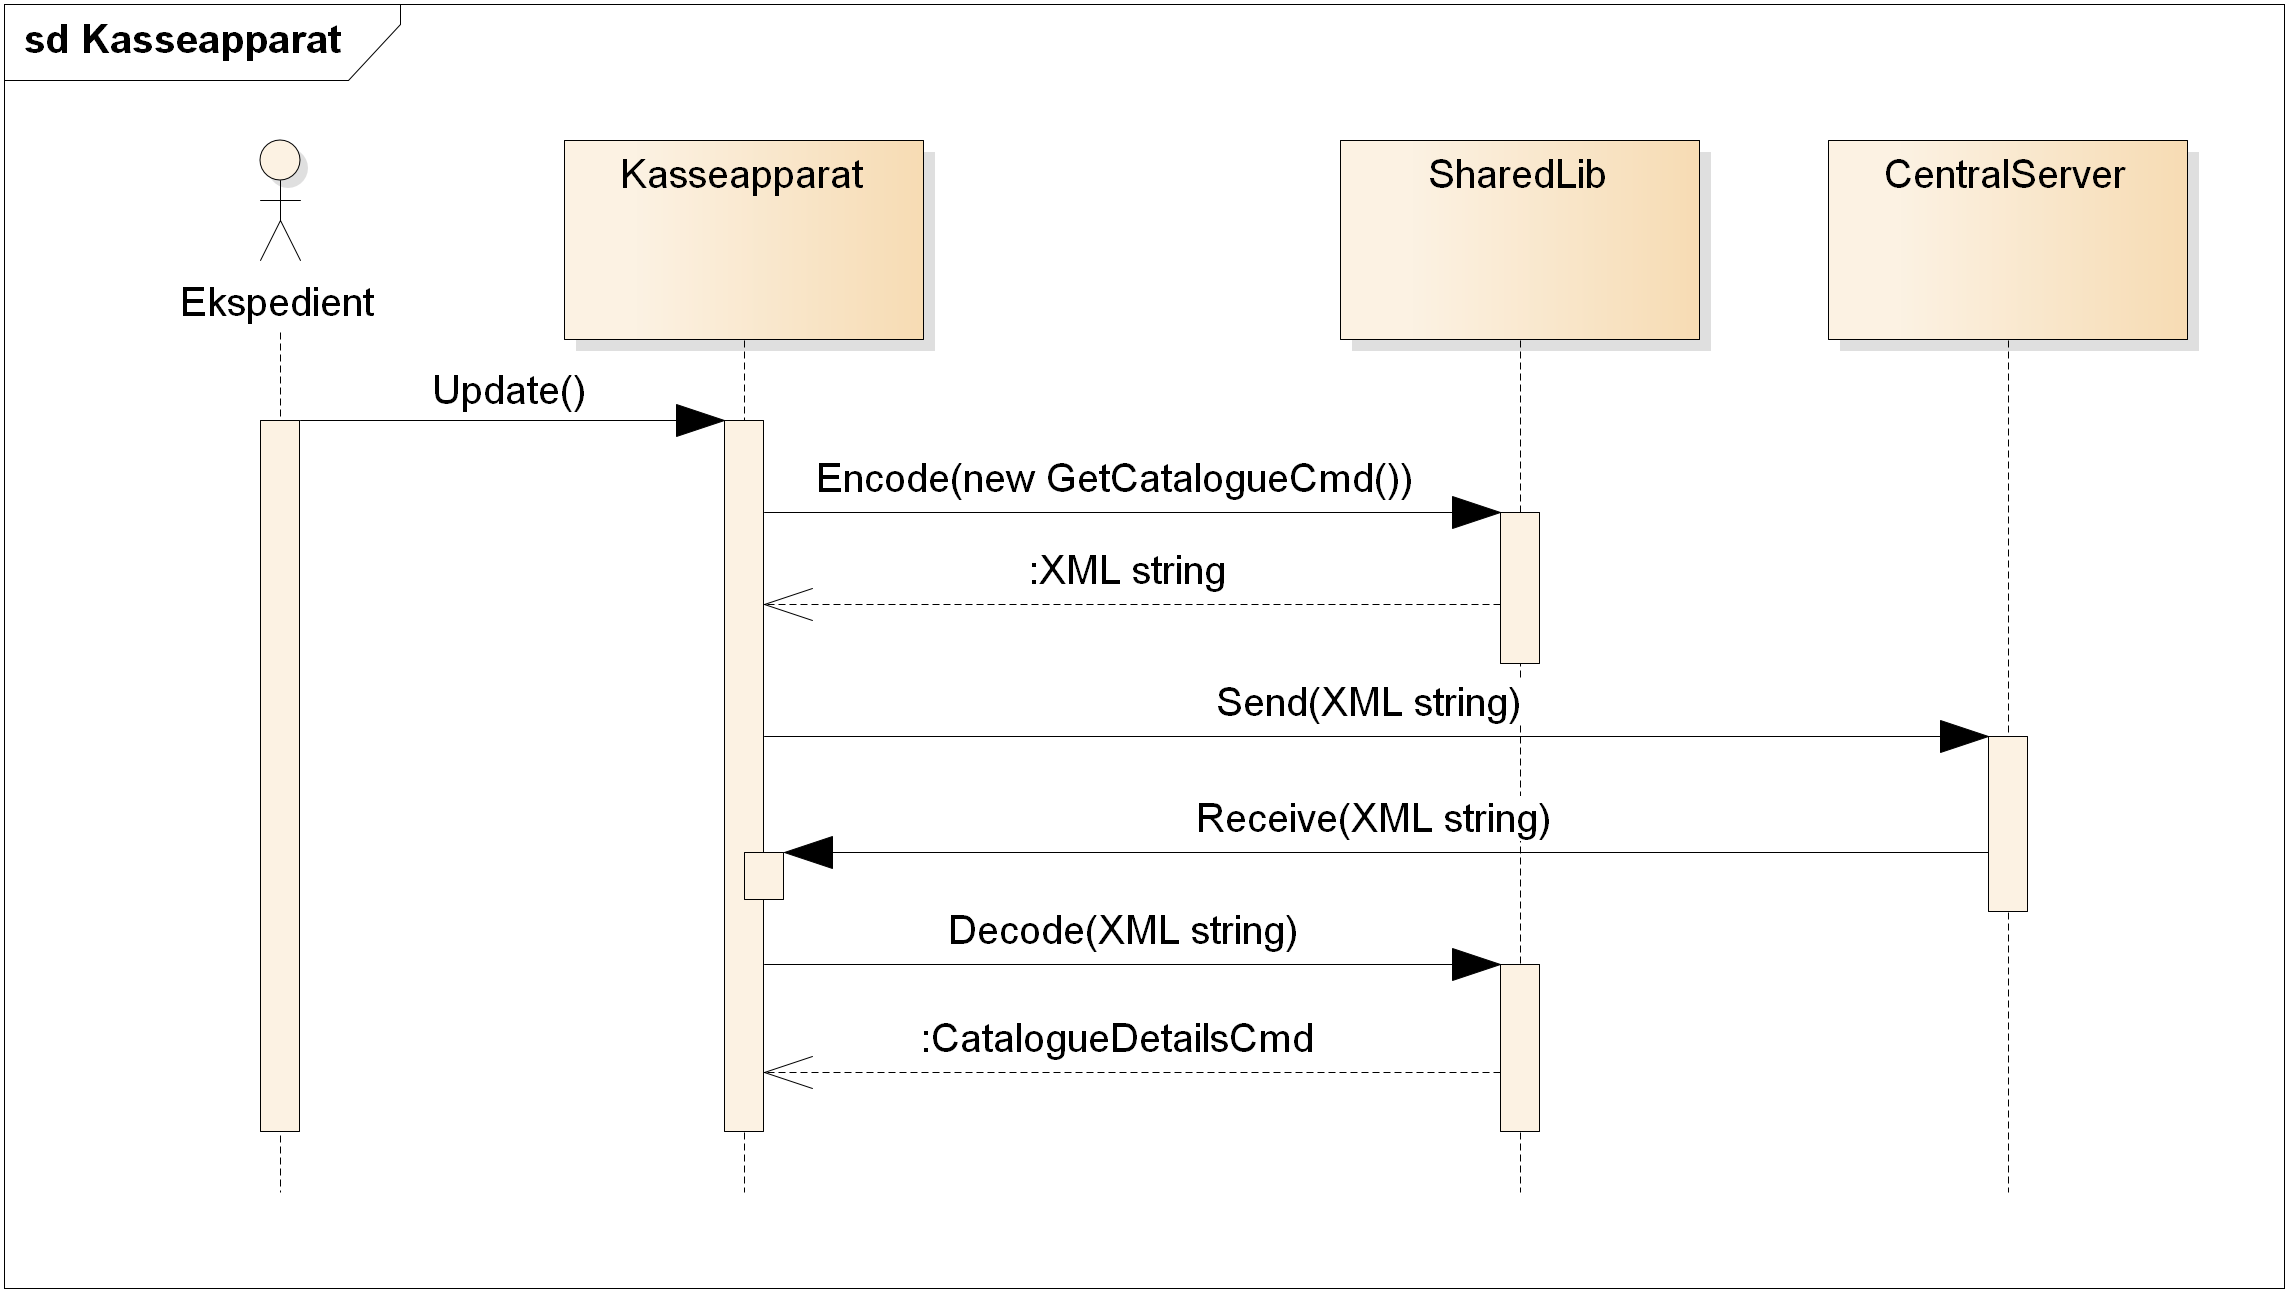
\includegraphics[width=\textwidth]{Systemarkitektur/LogiskView/Kasseapparat-sekvensdiagram}
	\caption{Sekvensdiagram for kommunikation mellem \gls{KA} og andre pakker}
	\label{fig:logview_kasse_sekvensdiagram}
\end{figure}

Sekvensdiagrammet viser hvordan \gls{KA} kommunikerer med de andre pakker i systemet. \gls{KA} kommunikerer udelukkende med \gls{CS}. Når \gls{KA} skal sende en besked til \gls{CS} bruger den \gls{SL} til at konvertere et kommando objekt til en XML string og sender herefter denne til \gls{CS}. Der modtages herefter en XML string, som respons, som så derefter bliver decoded til et kommando objekt, igen ved brug af \gls{SL}.

\newpage
